\chapter{Metais de transição e complexos de coordenação}\label{ch:b2:coordination-complexes}

Em 1893, um químico de vinte e seis anos, Alfred Werner, decidiu explicar um
enigma. O cloreto de cobalto(III) forma quatro compostos com a amônia,
\ce{CoCl3.6NH3}, \ce{CoCl3.5NH3} e dois de fórmula \ce{CoCl3.4NH3}, um verde e
um violeta. O nitrato de prata precipita de imediato os três cloretos do
primeiro, dois do segundo e apenas um de cada um dos dois últimos. A
resposta de Werner --- seis grupos mantidos em torno do metal nos vértices de
um octaedro, o resto do lado de fora --- fundou a química de coordenação.
Este capítulo estende os complexos do volume do 1.º ano à sua geometria, a
seus isômeros, a seus nomes e a uma contagem de elétrons que prevê quais
carbonilas metálicas existem.

\begin{recall}
O volume do 1.º ano: complexo, átomo central, ligante, ligante polidentado,
quelato, constantes de formação, número de coordenação; configurações
eletrônicas dos íons dos metais de transição (os elétrons $n$s perdidos
primeiro); ácidos e bases de Lewis, ligações dativas; VSEPR; números de
oxidação; enantiômeros. \Cref{ch:b2:atomic-orbitals}:
os orbitais d e a ordem dos níveis 4s e 3d.
\end{recall}

\begin{omfigure}
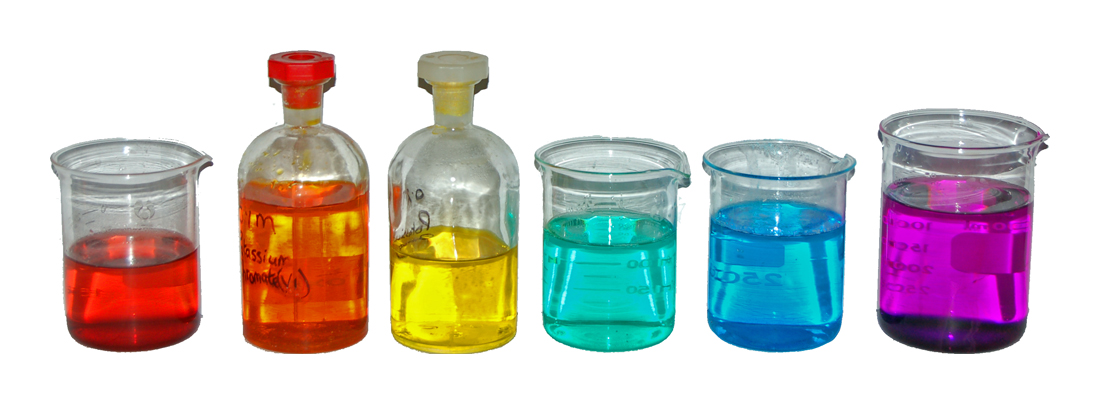
\includegraphics[width=0.8\linewidth]{images/book3/tm-solutions.jpg}

{\small Soluções aquosas de compostos de metais de transição: da esquerda para
a direita, nitrato de cobalto(II), dicromato de potássio, cromato de potássio,
cloreto de níquel(II), sulfato de cobre(II) e permanganato de potássio. As
cores das soluções de cobalto, níquel e cobre vêm de seus aquacomplexos.
(Fotografia: Benjah-bmm27, domínio público, Wikimedia Commons.)}
\end{omfigure}

\section{O bloco d}

\begin{definition}[Elemento de transição]\label{def:b2:coordination-complexes:transition-element}
Um \emph{elemento de transição}\index{elemento de transicao@elemento de transição} é um elemento cujo
átomo, ou um de cujos íons usuais, tem uma subcamada d parcialmente
preenchida. Um íon de um tal elemento com $n$ elétrons em seus orbitais d tem
uma \emph{configuração $d^n$}\index{configuracao dn@configuração $d^n$}.
\end{definition}

\begin{proposition}[Contagem dos elétrons d]\label{prop:b2:coordination-complexes:dn}
Um íon de metal de transição $\mathrm M^{m+}$ do grupo de número $g$ (3 a 12) tem uma
configuração $d^n$ com $n = g - m$.
\end{proposition}

\begin{proof}
O átomo neutro tem $g$ elétrons além do gás nobre precedente, nos orbitais $n$s
e $(n - 1)$d. Nos íons, os orbitais d ficam abaixo do orbital s
(\cref{ex:b2:atomic-orbitals:iron}): todos os $g - m$ elétrons de valência
restantes são elétrons d.
\end{proof}

Por exemplo, \ce{Fe^2+} (grupo 8) é $d^6$, \ce{Cu^2+} (grupo 11) $d^9$, \ce{Co^3+} (grupo 9)
$d^6$, \ce{Pt^2+} (grupo 10) $d^8$.

\section{Os ligantes}

\begin{definition}[Denticidade]\label{def:b2:coordination-complexes:denticity}
A \emph{denticidade}\index{denticidade} de um ligante é o número de seus átomos
ligados ao mesmo átomo central. Um \emph{ligante monodentado}\index{ligante monodentado} se
liga por um átomo (\ce{H2O}, \ce{NH3}, \ce{Cl-}, \ce{CO}); um \emph{ligante
bidentado}\index{ligante bidentado}, por dois (o etano-1,2-diamina, abreviado en; o
íon etanodioato, ox). Um \emph{ligante em ponte}\index{ligante em ponte} se liga a
dois átomos metálicos ao mesmo tempo. Um \emph{ligante ambidentado}\index{ligante ambidentado} pode se
ligar por um ou outro de dois átomos diferentes, como o íon nitrito (por N ou por
O) ou o tiocianato (por S ou por N).
\end{definition}

\begin{definition}[Esfera de coordenação]\label{def:b2:coordination-complexes:coordination-sphere}
A \emph{esfera de coordenação}\index{esfera de coordenacao@esfera de coordenação} de um complexo é o
conjunto do átomo central e dos ligantes ligados a ele, escrito entre
colchetes; os íons fora dos colchetes são contraíons, não ligados ao metal.
\end{definition}

\begin{omfigure}
\setchemfig{atom sep=2.2em}
\chemfig{M*5(-H_2N-CH_2-CH_2-NH_2-)}
\qquad
\chemfig{M*5(-O-(=O)-(=O)-O-)}
\qquad
\chemfig{N(-[:120]CH_2COO^{-})(-[:240]CH_2COO^{-})-CH_2-CH_2-N(-[:60]CH_2COO^{-})(-[:-60]CH_2COO^{-})}

\medskip
{\small Ligantes quelantes. À esquerda: o etano-1,2-diamina (en), bidentado por
seus dois nitrogênios. No meio: o íon etanodioato (ox), bidentado por dois
oxigênios. À direita: o ânion edta, que envolve um íon metálico com seus dois
nitrogênios e quatro oxigênios carboxilato (hexadentado).}
\end{omfigure}

\section{Números de coordenação e geometrias}

Dois, quatro e seis são os números de coordenação mais comuns. A prata(I) e o
ouro(I) dão complexos lineares (\ce{[Ag(NH3)2]+}); quatro ligantes formam um
tetraedro (\ce{[CoCl4]^2-}, \ce{[Zn(NH3)4]^2+}) ou um quadrado (\ce{[PtCl4]^2-},
\ce{[Ni(CN)4]^2-}); cinco, uma bipirâmide trigonal (\ce{Fe(CO)5}); seis, de longe
o caso mais frequente, um octaedro.

\begin{omfigure}
\begin{tikzpicture}[font=\small]
  \node[omligand] at (-0.8,0) {}; \node[omligand] at (0.8,0) {};
  \draw[thick, black!70] (-0.8,0) -- (0.8,0); \node[ommetal] at (0,0) {};
  \node at (0,-1.5) {linear, 2};
  \pic at (3,0) {omtetrahedron}; \node at (3,-1.5) {tetraédrico, 4};
  \pic at (6,0) {omsquareplanar}; \node at (6,-1.5) {quadrado plano, 4};
  \pic at (9,0) {omtbp}; \node[align=center] at (9,-1.65) {bipiramidal\\ trigonal, 5};
  \pic at (12,0) {omoctahedron}; \node at (12,-1.5) {octaédrico, 6};
\end{tikzpicture}

{\small As geometrias de coordenação comuns (metal em laranja, ligantes em
cinza; as ligações tracejadas apontam para trás da página).}
\end{omfigure}

O VSEPR, que coloca os pares de elétrons do átomo central o mais afastados
possível, falha aqui: um íon $d^8$ como \ce{Pt^2+} tem quatro pares de elétrons
d e quatro ligantes, e no entanto seus complexos são quadrados, e não
tetraédricos ou octaédricos. Os elétrons d não são pares localizados que
empurram os ligantes: suas energias dependem da geometria de um modo que o
próximo capítulo calcula.

\begin{proposition}[O $d^8$ quadrado plano]\label{prop:b2:coordination-complexes:square-planar}
Os complexos tetracoordenados dos íons $d^8$ da segunda e da terceira séries
de transição (\ce{Pd^2+}, \ce{Pt^2+}, \ce{Au^3+}) são quadrados planos.
\end{proposition}

\admitted

A explicação, o desdobramento dos níveis d pelos ligantes, vem no
\cref{ch:b2:ligand-field}.

\section{Isômeros}

\begin{definition}[Isômeros dos complexos]\label{def:b2:coordination-complexes:isomers}
Em um complexo octaédrico $\mathrm{MA_3B_3}$, o \emph{isômero fac}\index{isomero fac@isômero fac} tem
os três ligantes B em uma face do octaedro, e o \emph{isômero
mer}\index{isomero mer@isômero mer}, em um meridiano (três posições em um plano que passa
pelo metal). Os \emph{isômeros de ligação}\index{isomeros de ligacao@isômeros de ligação} diferem
pelo átomo pelo qual um \omterm{def:b2:coordination-complexes:denticity}{ligante ambidentado} se liga. Os \emph{isômeros de
ionização}\index{isomeros de ionizacao@isômeros de ionização} trocam um ligante com um contraíon, o
que dá íons diferentes em solução.
\end{definition}

\begin{proposition}[Contagem dos isômeros octaédricos]\label{prop:b2:coordination-complexes:isomer-count}
Em um octaedro, $\mathrm{MA_4B_2}$ tem dois isômeros (cis e trans), $\mathrm{MA_3B_3}$ dois
(fac e mer), e $\mathrm M(\mathrm{AA})_3$, com três \omterm{def:b2:coordination-complexes:denticity}{ligantes bidentados}, dois
enantiômeros, $\Delta$ e $\Lambda$.
\end{proposition}

\begin{proof}
Em um octaedro, duas posições quaisquer são adjacentes (cis, $90^\circ$) ou opostas
(trans, $180^\circ$): dois arranjos para os dois ligantes B. Para três ligantes B,
ou nenhum par está em trans (eles ocupam uma face: fac) ou exatamente um par
está em trans (o terceiro fica cis em relação aos dois: mer); três posições
mutuamente trans não existem. Para
$\mathrm M(\mathrm{AA})_3$, cada quelato ocupa duas posições cis; os três quelatos
se enrolam em torno do eixo de ordem três como as pás de uma hélice, girando
no sentido horário ou anti-horário quando vistos ao longo desse eixo: duas
imagens especulares, não sobreponíveis, já que o complexo não tem plano de
simetria.
\end{proof}

\begin{omfigure}
\begin{tikzpicture}[font=\scriptsize]
  \pic (a) at (0,0) {omoctahedron};
  \node[omligand, fill=omDef!70] at (a-L1) {}; \node[omligand, fill=omDef!70] at (a-L3) {};
  \node at (0,-1.5) {\small cis-$\mathrm{MA_4B_2}$};
  \pic (b) at (3,0) {omoctahedron};
  \node[omligand, fill=omDef!70] at (b-L1) {}; \node[omligand, fill=omDef!70] at (b-L2) {};
  \node at (3,-1.5) {\small trans-$\mathrm{MA_4B_2}$};
  \pic (c) at (6.5,0) {omoctahedron};
  \node[omligand, fill=omThm!70] at (c-L1) {}; \node[omligand, fill=omThm!70] at (c-L3) {}; \node[omligand, fill=omThm!70] at (c-L5) {};
  \node at (6.5,-1.5) {\small fac-$\mathrm{MA_3B_3}$};
  \pic (d) at (9.5,0) {omoctahedron};
  \node[omligand, fill=omThm!70] at (d-L1) {}; \node[omligand, fill=omThm!70] at (d-L2) {}; \node[omligand, fill=omThm!70] at (d-L3) {};
  \node at (9.5,-1.5) {\small mer-$\mathrm{MA_3B_3}$};
\end{tikzpicture}

\medskip
\begin{tikzpicture}[font=\scriptsize]
  \foreach \xs/\s/\lab in {0/1/{$\Delta$}, 4.5/-1/{$\Lambda$}} {
    \begin{scope}[xshift=\xs cm, xscale=\s]
      \draw[black!30] (0,0) circle (1.2);
      \foreach \a in {90, 210, 330} {
        \coordinate (p) at (\a:1.1); \coordinate (q) at (\a+70:0.55);
        \draw[very thick, omDef] (\a:1.1) .. controls (\a+30:1.25) and (\a+60:0.9) .. (\a+75:0.55);
        \node[omligand] at (\a:1.1) {}; \node[omligand] at (\a+75:0.55) {};
      }
      \node[ommetal] at (0,0) {};
    \end{scope}
    \node at (\xs,-1.6) {\small \lab};
  }
  \draw[densely dashed] (2.25,-1.3) -- (2.25,1.3);
  \node[anchor=south] at (2.25,1.3) {espelho};
\end{tikzpicture}

{\small Em cima: isômeros cis e trans de $\mathrm{MA_4B_2}$ (ligantes B em azul),
\omterm{def:b2:coordination-complexes:isomers}{isômeros fac} e mer de $\mathrm{MA_3B_3}$ (B em vermelho). Embaixo: os dois
enantiômeros de um tris-quelato como \ce{[Co(en)3]^3+}, vistos ao longo do eixo
de ordem três, esquemáticos: cada quelato (arco azul) une uma posição superior
e uma inferior, e os três giram em um sentido ($\Delta$) ou no outro
($\Lambda$).}
\end{omfigure}

\section{Nomes e contagem de elétrons}

\begin{method}[Nomear um complexo]\label{met:b2:coordination-complexes:naming}
\begin{enumerate}
  \item Na fórmula, escreva a \omterm{def:b2:coordination-complexes:coordination-sphere}{esfera de coordenação} entre colchetes, primeiro o
        metal, depois os ligantes; a carga do complexo fica do lado de fora.
  \item No nome, liste os ligantes em ordem alfabética com prefixos
        multiplicativos (di-, tri-, tetra-; bis-, tris- para nomes de ligantes
        complexos): os ligantes aniônicos terminam em -o (clorido, cianido,
        óxido, hidróxido), os neutros conservam seus nomes (aqua, amin,
        carbonil).
  \item Depois vem o metal, com a terminação -ato se o complexo for um ânion
        (ferrato, cuprato, cobaltato), e seu número de oxidação em algarismos
        romanos.
  \item Em português, o ânion é nomeado primeiro, ligado ao cátion por
        ``de'': \ce{[Co(NH3)6]Cl3} é o cloreto de hexa-amincobalto(III), e
        \ce{K4[Fe(CN)6]}, o hexacianidoferrato(II) de potássio.
\end{enumerate}
\end{method}

\begin{definition}[Contagem de elétrons]\label{def:b2:coordination-complexes:electron-count}
A \emph{contagem de elétrons de valência}\index{contagem de eletrons de valencia@contagem de elétrons de valência} de um complexo é
o número de elétrons d do íon metálico mais os elétrons cedidos pelos ligantes
(dois para cada par doador). A \emph{regra dos 18 elétrons}\index{regra dos 18 eletrons@regra dos 18 elétrons} afirma
que os complexos estáveis de metais em baixo estado de oxidação com ligantes
$\pi$-aceptores fortemente ligados, como \ce{CO}, tendem a ter 18 elétrons de
valência.
\end{definition}

\begin{definition}[Hapticidade]\label{def:b2:coordination-complexes:hapticity}
A \emph{hapticidade}\index{hapticidade} de um ligante é o número de seus átomos
ligados ao metal por um mesmo sistema $\pi$ contínuo; ela é escrita $\eta^n$: um
eteno ligado por sua ligação $\pi$ é $\eta^2$; um anel ciclopentadienila ligado
pelos cinco carbonos, $\eta^5$.
\end{definition}

\begin{method}[Contar os elétrons]\label{met:b2:coordination-complexes:electron-count}
\begin{enumerate}
  \item Atribua cargas aos ligantes como espécies de camada fechada (\ce{Cl-}, \ce{H-},
        \ce{C5H5-}; \ce{CO}, \ce{PR3}, \ce{NH3} neutros) e deduza o estado de
        oxidação do metal.
  \item Conte os elétrons d do metal, $n = g - m$.
  \item Some dois elétrons por par doador: um par por \omterm{def:b2:coordination-complexes:denticity}{ligante monodentado},
        seis elétrons para um $\eta^5$-\ce{C5H5-}, seis para um $\eta^6$-benzeno,
        dois para um $\eta^2$-alceno.
  \item Uma ligação metal--metal conta um elétron para cada metal.
\end{enumerate}
\end{method}

\begin{proposition}[Carbonilas metálicas]\label{prop:b2:coordination-complexes:eighteen}
As carbonilas binárias estáveis da primeira série de transição, \ce{Cr(CO)6},
\ce{Fe(CO)5}, \ce{Ni(CO)4} e \ce{Mn2(CO)10}, têm todas 18 elétrons de valência
por átomo metálico.
\end{proposition}

\begin{proof}
Cromo(0), $d^6$, com seis CO: $6 + 12 = 18$. Ferro(0), $d^8$, cinco CO: $8 + 10 = 18$.
Níquel(0), $d^{10}$, quatro CO: $10 + 8 = 18$. Manganês(0), $d^7$, cinco CO e uma
ligação Mn--Mn: $7 + 10 + 1 = 18$; um \ce{Mn(CO)5} monomérico, com 17, não existe
como composto estável e se emparelha. A razão pela qual 18 é favorecido ---
nove orbitais de valência do metal, todos os ligantes ou não ligantes
preenchidos --- é dada no \cref{ch:b2:ligand-field}.
\end{proof}

O ferroceno, \ce{Fe(\eta^5-C5H5)2}, mantém um íon ferro(II) ($d^6$) entre dois
ânions ciclopentadienila, cada um cedendo seis elétrons: $6 + 12 = 18$. A regra
falha para a maioria dos complexos de estados de oxidação altos e para muitos
com ligantes fracos: \ce{[Ti(H2O)6]^3+} tem 13 elétrons, \ce{[Cu(H2O)6]^2+} 21.

\begin{history}[Werner e o octaedro]
\begin{minipage}[t]{0.22\linewidth}
\vspace{0pt}
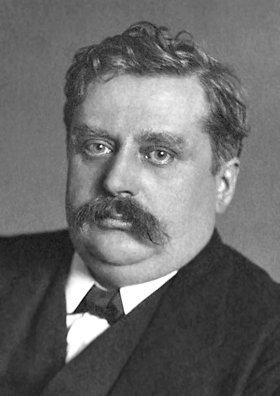
\includegraphics[width=\linewidth]{images/book3/werner.jpg}
\end{minipage}\hfill
\begin{minipage}[t]{0.74\linewidth}
\vspace{0pt}
Alfred Werner propôs em 1893 que um metal tem, além de sua valência, um número
de coordenação de grupos mantidos diretamente à sua volta, e que o
cobalto(III) mantém seis deles nos vértices de um octaedro. Ele previu então
quantos isômeros cada fórmula deveria ter e passou vinte anos preparando-os;
em 1911, resolveu um complexo de cobalto em seus dois enantiômeros, provando
que a quiralidade não exige um átomo de carbono. Recebeu o Prêmio Nobel de
Química em 1913. (Retrato, Les Prix Nobel, 1914, domínio público, Wikimedia
Commons.)
\end{minipage}
\end{history}

\section{Exercícios}

\begin{exercise}[$\star$]\label{exo:b2:coordination-complexes:1}
Dê a configuração $d^n$ de \ce{Ti^3+}, \ce{V^3+}, \ce{Cr^3+}, \ce{Mn^2+}, \ce{Fe^3+},
\ce{Co^2+}, \ce{Ni^2+} e \ce{Zn^2+}.
\end{exercise}

\begin{exercise}[$\star$]\label{exo:b2:coordination-complexes:2}
Dê a \omterm{def:b2:coordination-complexes:denticity}{denticidade} da água, do etano-1,2-diamina, do íon etanodioato, do edta e
do íon tiocianato, e diga qual é ambidentado.
\end{exercise}

\begin{exercise}[$\star$]\label{exo:b2:coordination-complexes:3}
Dê o nome de \ce{[Cu(NH3)4]SO4}, \ce{K3[Fe(CN)6]}, \ce{[CoCl2(NH3)4]Cl} e
\ce{[Ni(CO)4]}.
\end{exercise}

\begin{exercise}[$\star$]\label{exo:b2:coordination-complexes:4}
Preveja a geometria de \ce{[Ag(NH3)2]+}, \ce{[CoCl4]^2-}, \ce{[PtCl4]^2-} e
\ce{[Fe(H2O)6]^2+}.
\end{exercise}

\begin{exercise}[$\star\star$]\label{exo:b2:coordination-complexes:5}
Quantos isômeros tem o \ce{[PtCl2(NH3)2]} quadrado plano? Desenhe-os. (Um deles,
a cisplatina, é um medicamento anticâncer.)
\end{exercise}

\begin{exercise}[$\star\star$]\label{exo:b2:coordination-complexes:6}
Conte os elétrons de valência de \ce{Cr(CO)6}, \ce{Fe(CO)5}, \ce{Ni(CO)4},
\ce{V(CO)6} e \ce{Mn2(CO)10}. Qual deles viola a regra, e como ele se comporta?
\end{exercise}

\begin{exercise}[$\star\star$]\label{exo:b2:coordination-complexes:7}
Conte os elétrons de valência do ferroceno e do cobaltoceno \ce{Co(C5H5)2}. Qual
é facilmente oxidado, e a quê?
\end{exercise}

\begin{exercise}[$\star\star$]\label{exo:b2:coordination-complexes:8}
O complexo de níquel(II) do edta tem $\log_{10}K = 20.5$, muito acima do de
complexos nos quais o níquel se liga a seis doadores nitrogênio ou oxigênio
separados. Explique esse efeito quelato pelo número de partículas liberadas
quando o quelato substitui seis moléculas de água.
% ledger: logb:Ni-edta
\end{exercise}

\begin{exercise}[$\star\star$]\label{exo:b2:coordination-complexes:9}
Desenhe os dois \omterm{def:b2:coordination-complexes:isomers}{isômeros de ligação} de \ce{[Co(NO2)(NH3)5]^2+}.
\end{exercise}

\begin{exercise}[$\star\star\star$]\label{exo:b2:coordination-complexes:10}
Quantos estereoisômeros tem \ce{[CoCl2(en)2]+}? Quais são quirais?
\end{exercise}

\begin{exercise}[$\star\star\star$]\label{exo:b2:coordination-complexes:11}
Para $\mathrm{MA_4B_2}$, conte os isômeros previstos por um hexágono plano e por um
prisma trigonal de seis ligantes, e explique como o número de isômeros
encontrados permite decidir entre as geometrias.
\end{exercise}

\begin{exercise}[$\star\star\star$]\label{exo:b2:coordination-complexes:12}
Conte os elétrons de valência de \ce{[RhCl(PPh3)3]} e de \ce{[IrH(CO)(PPh3)3]}
(\ce{PPh3} um doador de dois elétrons, \ce{H-} como hidreto). Qual deles poderia
receber mais dois ligantes?
\end{exercise}

\section{Problema: As aminas de cobalto de Werner}

\begin{problem}[{Problema de fim de semana --- quatro aminas de cloreto de cobalto(III) e
o cloreto que elas liberam, suas fórmulas com colchetes, os dois isômeros da
tetra-amina e o que eles provam sobre a geometria, e a atividade óptica de um
tris-quelato}]
\label{pb:b2:coordination-complexes:1}
Dados: quatro compostos, A \ce{CoCl3.6NH3} (amarelo-alaranjado), B \ce{CoCl3.5NH3}
(púrpura), C e D \ce{CoCl3.4NH3} (verde e violeta). Com excesso de nitrato de
prata, um mol de A precipita 3 mol de \ce{AgCl}, B 2 mol, C e D 1 mol cada um.
As condutividades molares indicam 4, 3, 2 e 2 íons por unidade de fórmula.

\medskip
\noindent\textbf{Parte I --- Cloreto e íons.}
\begin{enumerate}
  \item Quais cloretos reagem de imediato com os íons prata?
  \item Quantos cloretos estão ligados ao cobalto em cada composto?
  \item Confronte os números de íons com as condutividades.
  \item Qual é o número de oxidação do cobalto nos quatro?
  \item Qual é sua configuração $d^n$?
  \item Que número total de ligantes o cobalto mantém em cada composto?
\end{enumerate}

\medskip
\noindent\textbf{Parte II --- Fórmulas e nomes.}
\begin{enumerate}[resume]
  \item Escreva A, B, C e D com colchetes.
  \item Dê o nome de A e de B.
  \item Dê o nome do cátion de C e D.
  \item Que tipo de isômeros são C e D?
  \item O que seria um composto \ce{CoCl3.3NH3}, e quantos íons ele daria?
  \item Quantos isômeros esse composto teria em um octaedro?
\end{enumerate}

\medskip
\noindent\textbf{Parte III --- A geometria.}
\begin{enumerate}[resume]
  \item Desenhe os \ce{[CoCl2(NH3)4]+} cis e trans em um octaedro.
  \item Conte os isômeros de \ce{[CoCl2(NH3)4]+} previstos para seis ligantes
        nos vértices de um hexágono plano.
  \item Conte os previstos para um prisma trigonal.
  \item Werner nunca encontrou mais de dois. O que isso prova?
  \item A prova é completa? O que teria significado um terceiro isômero?
  \item Qual de C e D é o cis, sabendo que o isômero cis pode ser convertido em
        um quelato com etanodioato e o trans não?
\end{enumerate}

\medskip
\noindent\textbf{Parte IV --- A atividade óptica.}
\begin{enumerate}[resume]
  \item Desenhe \ce{[Co(en)3]^3+}.
  \item Ele tem um plano de simetria? Um centro de inversão?
  \item Quantos estereoisômeros ele tem?
  \item O que prova a resolução de um tal cátion em enantiômeros?
  \item O \ce{[CoCl2(en)2]+} é quiral em sua forma cis? Em sua forma trans?
  \item Por que a resolução, por Werner, de um complexo que não contém carbono
        algum foi importante?
  \item Dê o número de isômeros de \ce{[CoCl2(NH3)4]+} previsto pelo octaedro, e
        pelo hexágono plano e pelo prisma trigonal.
\end{enumerate}
\end{problem}
